\chapter{Evaluierung}\label{kap:eval}

Bevor die Ergebnisse der trainierten Modell diskutiert 
werden, behandelt dieses Kapitel zunächst einige der für die 
Objekterkennung üblicherweiser verwendeten Metriken zur Messung
der Genauigkeit. 


Anschließend werden die Modell in \ref{sec:model_vergleich}
miteinander verglichen und in \ref{sec:optimierung_faster_rcnn}
optimierungsverfahren für das Faster R-CNN Model ausgewertet.


\section{Evaluierungs Metriken}\label{sec:metricen}

\subsection*{Mean Average Precision (mAP)}

Als Metrik für die Genauigkeit eines Object Detection Models 
dient die \textit{Mean Average Precision (mAP)}, welche 
sowohl Klassifizierung als auch Lokalisierung mit einbezieht 
und sich aus folgenden Werten berechenn lässt.


\begin{itemize}
  \item \textit{True Positive (TP)}: 
  \item \textit{True Negative (TN)}: 
  \item \textit{False Positive (FP)}: 
  \item \textit{False Negative (FN)}: 
\end{itemize}

Zur bestimmung dieser Werte wird die \textit{Intersection over unioun}
verwendet, welche Überlappungsgrad der gelabelten (Ground Truth) und der
geschätzete Boundig Box zu dem Gesammtbereich beider Boxen darstellt 

Beträgt dieser mehr als ein Bestimmter Threshhold, häufig 50\%
gilt die Schätzung als \textit{True Positive}, andernfalls als 
\textit{False Positive}. 


% für confusion matrix
\newcommand\MyBox[2]{
  \fbox{\lower0.75cm
    \vbox to 1.7cm{\vfil
      \hbox to 1.7cm{\hfil\parbox{1.4cm}{#1\\#2}\hfil}
      \vfil}%
  }%
}
\noindent
\renewcommand\arraystretch{1.5}
\setlength\tabcolsep{0pt}

\begin{minipage}{\textwidth}
    \begin{minipage}[b]{0.49\textwidth}
      \centering
      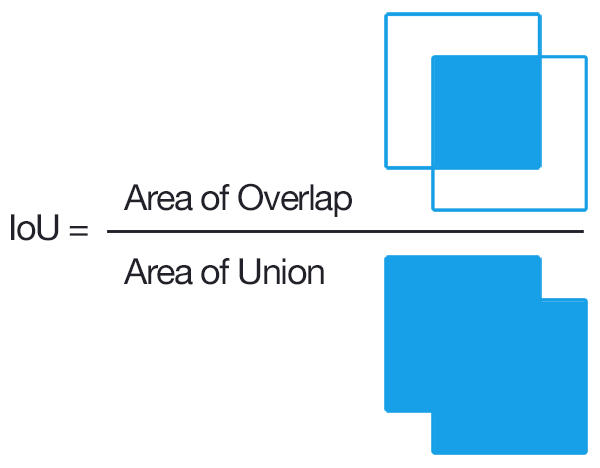
\includegraphics[width=0.8\textwidth]{Bilder/IoU.png}
      \captionof{figure}{Intersection over Union}
    \end{minipage}
    \hfill
    \begin{minipage}[b]{0.49\textwidth}
      \centering
      \begin{tabular}{c >{\bfseries}r @{\hspace{0.7em}}c @{\hspace{0.4em}}c @{\hspace{0.7em}}l}
        \multirow{10}{*}{\rotatebox{90}{\parbox{2.5cm}{\bfseries\centering tatsächlicher Wert}}} & 
          & \multicolumn{2}{c}{\bfseries geschätzter Wert} & \\
        & & \bfseries p & \bfseries n & \bfseries\\
        & p$'$ & \MyBox{True}{Positive} & \MyBox{False}{Negative}\\[2.4em]
        & n$'$ & \MyBox{False}{Positive} & \MyBox{True}{Negative} \\
      \end{tabular}
        \captionof{figure}{Confusion Matrix}
    \end{minipage}
\end{minipage}


\vspace{0.5cm}
    
Daraus lassen sich dann Precision und Recall berechnen. 

\textit{Recall}
welcher angibt wie 
viele Objekte das Modell gefunden hat
\begin{equation}
  Recall = \frac{TP}{TP + FN}
\end{equation}
TP + FN allen Objekten im Bild entspricht, somit also das 
Verhälltnis der Gefunden zu allen Objekten im Bild


\textit{Precision}
die angibt mit welcher Genauigkeit die Objekte gefunden wurden
\begin{equation}
  Precision = \frac{TP}{TP + FP}
\end{equation}
also die richtig 
geschätzen durch alle gemachten schätzunge und gibt somit die 
genauigkeit mit der das Model die Objekte findet an.


\textit{Average Precision}
\begin{equation}
  Average Precision = \frac{1}{N}\sum(Precision(Recall))
\end{equation}

Daraus kann nun die durchschnittliche Precision für alle Recall 
Werte bestimmt werden, welche als \textit{Average Precision}
bezeichnet wird und die Genauigkeit des Models bezogen auf 
eine bestimmte Klasse angibt

\textit{mean Average Precision}
Für alle Klassen gemittel 
erhält man die mittlere durchschnittliche Precision (mAP)



\subsection*{Fehlerfunktion (Loss)}
Die Fehlerfunktion setzet sich aus einem Lokalisierungs und einem 
Klassifizierungsfehler zusammen. 
Die Lokalisierung erfolgt über eine Lineare Regression zur 
Annäherung der Bounding Boxes and die richtigen Koordinaten.\\

Bei Faster R-CNN werden diese beiden Loss Werte dann sowohl für 
RPN(1st stage) als auch für classifier(2nd stage) also 
insgesammt 4 loss werte verwendet.



%----------------- SECTION: validtaion ---------------------
\section{Vergleich der Modelle}\label{sec:model_vergleich}
In diesem Abschnitt werden die beiden für das Training verwendeten
Objec Detection Architekturen Single Shot Detector (SSD)
und Faster R-CNN miteinander verglichen.



\subsection{Evaluierung/Validierung}

Die Evaluierungsergebnisse beziehen sich auf das 
Testsets aus dem Open Images Datensatz.
\\
SSD wurd mit Batchsize=12 75k durchläufe trainiert.\\
Faster R-CNN mit Batchsize=1 für 200k durchläufe.(1 weil dynamische input size)\\
eine epoche sind (teps mal batchsize)/samples
\\
\begin{table}[H]
  \centering
  \begin{tabular}{m{0.25\textwidth}m{0.2\textwidth}|m{0.15\textwidth}<{\centering}m{0.15\textwidth}<{\centering}}
  \hline
  Model                                                              & Optimierung                                                                   & mAP                                                        & Loss                                                       \\ \hline\hline
  SSD + MobilenetV2                                                  & \begin{tabular}[c]{@{}l@{}}Ohne\\ Augmentierung\end{tabular}                  & \begin{tabular}[c]{@{}l@{}}0,62\\ 0,61\end{tabular}        & \begin{tabular}[c]{@{}l@{}}3,56\\ 3,50\end{tabular}        \\ \hline
  SSD + InceptionV2                                                  & \begin{tabular}[c]{@{}l@{}}Ohne\\ Augmentierung\end{tabular}                  & \begin{tabular}[c]{@{}l@{}}0,65\\ 0,62\end{tabular}        & \begin{tabular}[c]{@{}l@{}}3,86\\ 3,71\end{tabular}        \\ \hline
  \begin{tabular}[c]{@{}l@{}}Faster R-CN\\ +InceptionV2\end{tabular} & \begin{tabular}[c]{@{}l@{}}Ohne\\ Augmentierung\\ Early Stopping\end{tabular} & \begin{tabular}[c]{@{}l@{}}0,67\\ 0,69\\ 0,67\end{tabular} & \begin{tabular}[c]{@{}l@{}}0,82\\ 0,67\\ 0,69\end{tabular} \\ \hline
  \end{tabular}
\end{table}

Man kann erkennen das der Feler (Loss) durch Augmentierung etwas 
veringert wurde.
Insbesondere beim Faster R-CNN, welches aufgrund der 
höheren komplexität, schneller zur überanpassung neigt.\\
Der Verlauf des Trainings ließ sich mihilfe des Evaluierungstools Tensorboard
Visualisieren, Plots für die drei Konfigurationen des Faster R-CNN sind in 
Abbildung \ref{plot:mAP} und \ref{plot:loss} dargestellt.
\vspace{0.5cm}

\begin{figure}[htb]
\begin{minipage}{0.5\textwidth}
  \centering
  \label{plot:mAP}
  \def\svgwidth{0.9\textwidth}
  \input{Bilder/plots/overfitting_kein_early_aug_mAP.pdf_tex}
  \captionof{figure}{mAP}
\end{minipage}
\begin{minipage}{0.5\textwidth}
  \centering
  \label{plot:Loss}
  \def\svgwidth{0.9\textwidth}
  \input{Bilder/plots/overfitting_kein_early_aug_loss.pdf_tex}
  \captionof{figure}{Loss}
\end{minipage}
\end{figure}

% Legende: Overfitting
\begin{table}[htb]
  \centering
  \begin{tabular}{m{0.1\textwidth}<{\centering}m{0.2\textwidth}<{\centering}m{0.2\textwidth}<{\centering}}
    $\color[HTML]{FF7043}\medbullet$  Ohne & $\color[HTML]{0077BB}\medbullet$  Early Stopping & $\color[HTML]{CC3311}\medbullet$  Augmentierung
  \end{tabular}    
\end{table}

% colors
% orange: FF7043
% blue  : 0077BB
% red   : CC3311



hier die zwi techniken zur vermeidung von overfitting: augmentierung
und Loss gegenübergestellt. Augmentierung erzielt bessere ergebnisse, 
da durch vorzeitiges stoppen des trainings auch keine weitere verbesserung
bezüglich mAP mehr stattfinden konnte.

% weitere Beobachtung: wenn eval für anderes Datenset 
% angewendet wird ist auch der Loss des Augmentierten 
% Datensets besser.



%----------------- SECTION: Test Inferenz ---------------------
\subsection{Test Inferenz}\label{sec:test_inferenz}

Um eine bessere Vorstellung davon zu bekommen wie sich die 
unterschiedlichen Ergebnisse in mAP und Loss in der Anwendung 
tatsächlich bemerkbar machen, wurde die Inferenz der drei modelle 
für verschiedene Test Bilder durchgeführt.

Dafür wurden die Modelle in die für OpenVino benötigte Intermediate
Representation umgewandelt um dann mihilfe eines Python 
Scripts in die InferenceEngine geladen zu werden.

Mithilfe dieses Scripts konnten nun die Inferenz für 
folgende Testszenarien:

\begin{itemize}
  \item inferenz auf Test Set \textit{OpeImages}
  \item inferenz auf \textit{The iWildCam 2019 Dataset}\cite{beery2019iwildcam}
  \item inferenz auf eigene Bilder
\end{itemize}


\subsubsection{Test Set (OpenImages)}
Sowohl SSD als auch Faster R-CNN erkennen das meiste, da gr 
ähnlichkeit zu Trainingssatz.

Wenn jedoch mehrere Tiere im Bild sind, diese weiter weg oder schlechtere
Bildqualität, erkennt Faster R-CNN besser. Abb \ref{fig:faster_rcnn}
\\[1cm]
\begin{minipage}{0.5\textwidth}
  \centering
  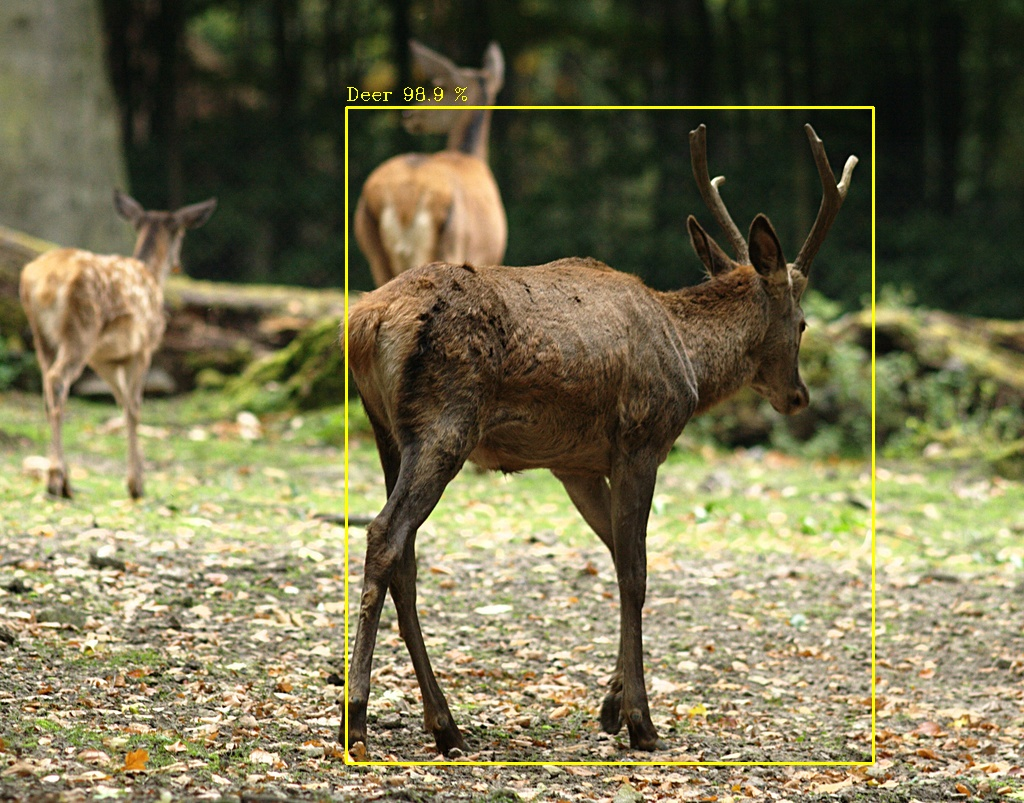
\includegraphics[width=0.9\textwidth]{model_compare_test__ssd_inception_v2.jpg}
  \captionof{figure}{SSD}
  \label{fig:ssd}
\end{minipage}
\begin{minipage}{0.5\textwidth}
  \centering
  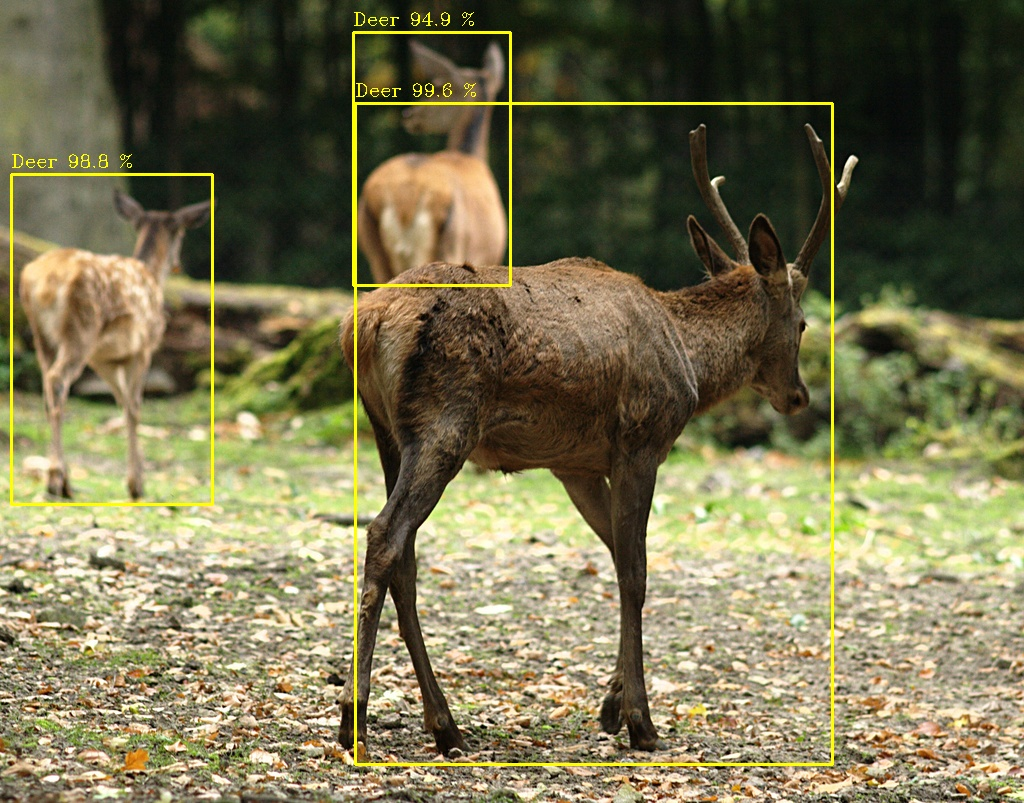
\includegraphics[width=0.9\textwidth]{model_compare_test__faster_rcnn_inception_v2_early_stopping.jpg}
  \captionof{figure}{Faster R-CNN}
  \label{fig:faster_rcnn}
\end{minipage}


\subsubsection{Eigene Aufnahmen}

\begin{minipage}{0.5\textwidth}
  \centering
  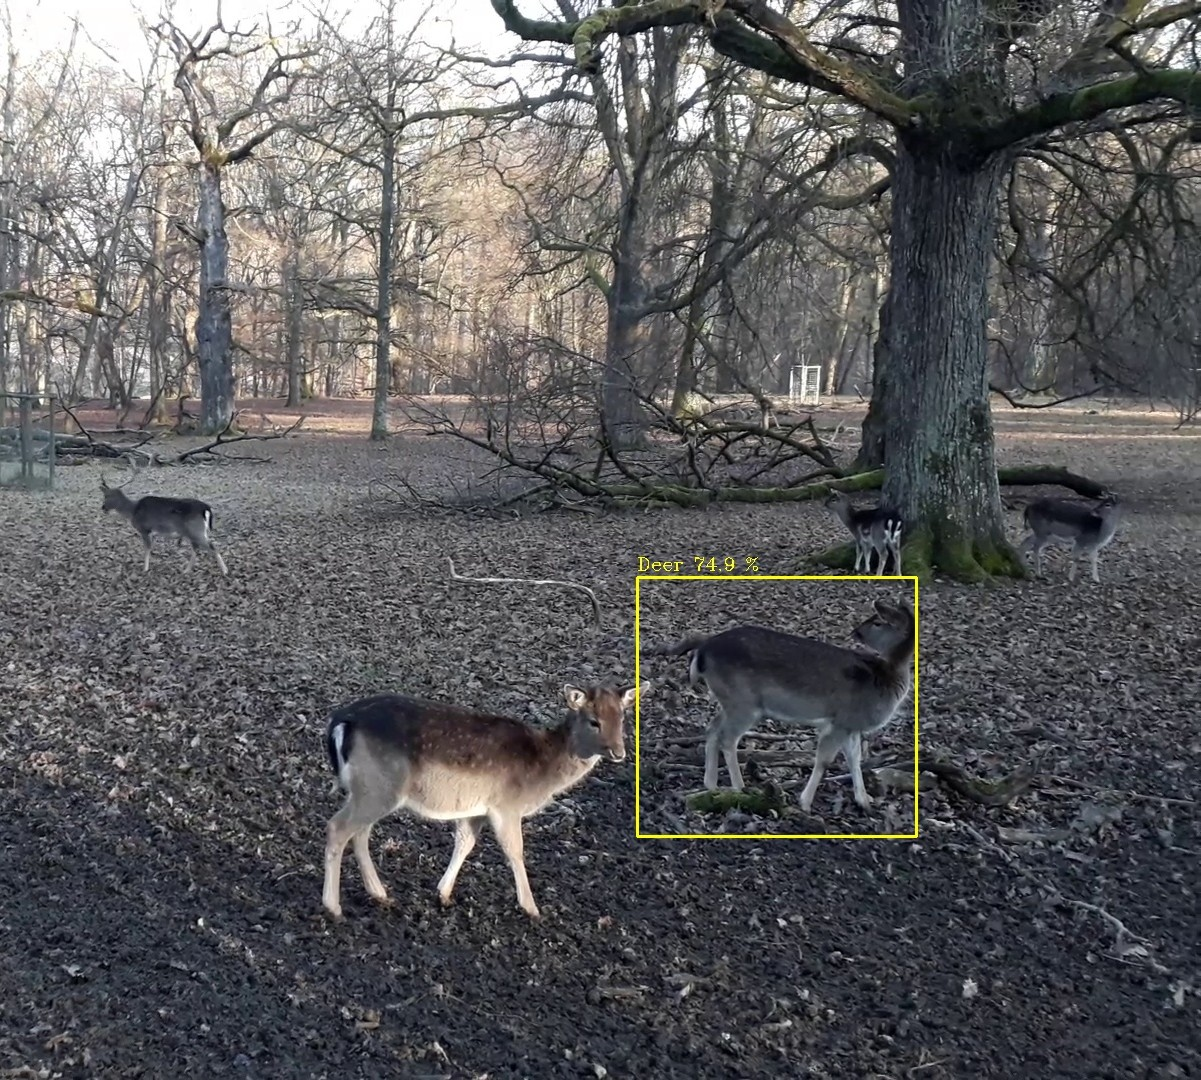
\includegraphics[width=0.9\textwidth]{model_compare_handy_ssd_mobilenet_v2.jpg}
  \captionof{figure}{SSD Mobilnet}
  \label{}
\end{minipage}
\begin{minipage}{0.5\textwidth}
  \centering
  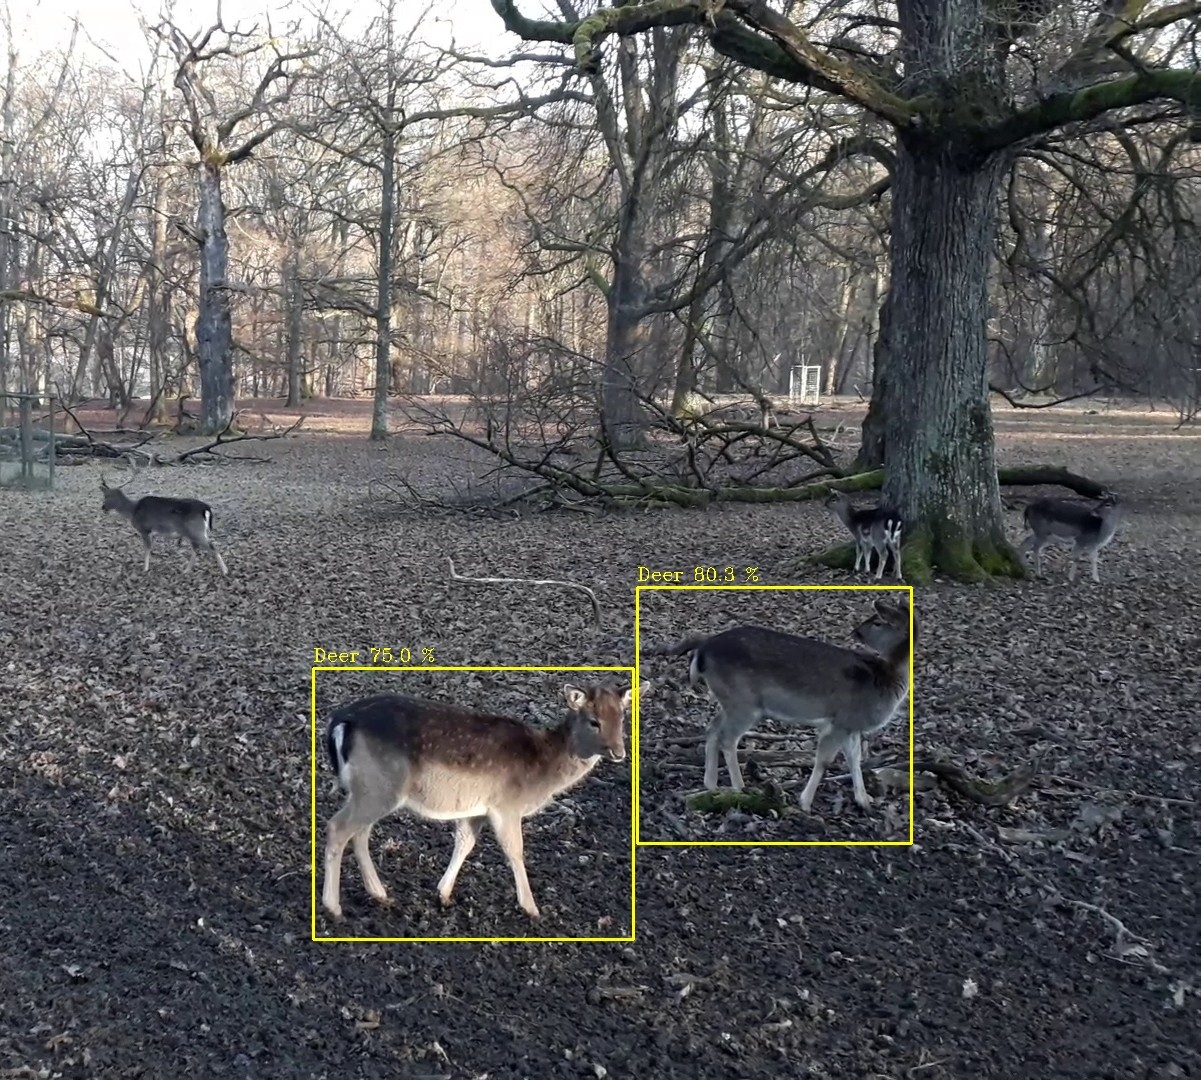
\includegraphics[width=0.9\textwidth]{model_compare_handy_ssd_inception_v2.jpg}
  \captionof{figure}{SSD Inception}
  \label{}
\end{minipage}
\\[1cm]
\begin{minipage}{0.5\textwidth}
  \centering
  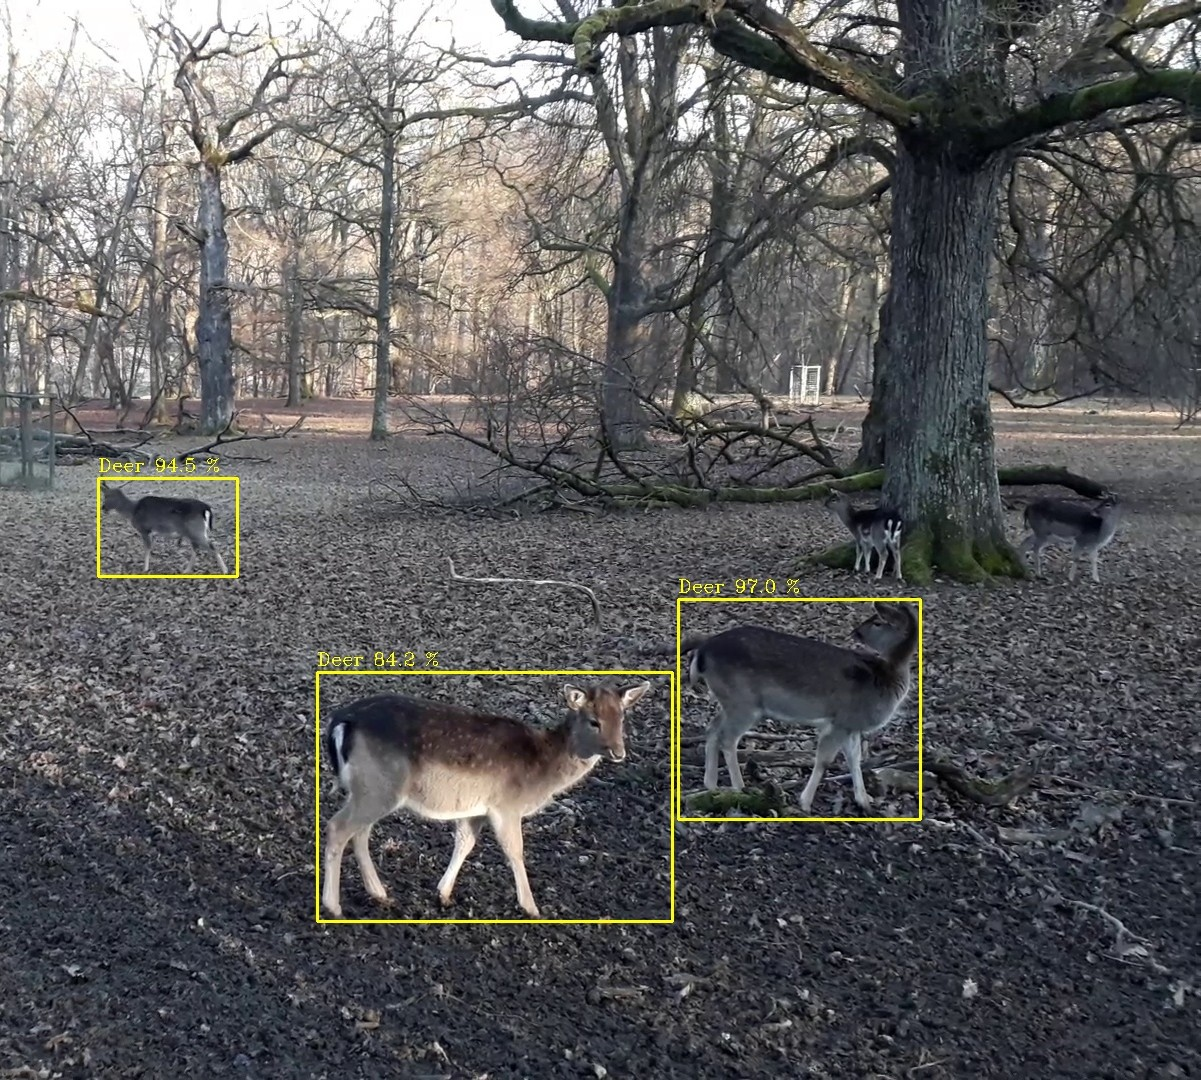
\includegraphics[width=0.9\textwidth]{model_compare_handy_faster_rcnn_inception_v2_early_stopping_ohne_aug.jpg}
  \captionof{figure}{Faster R-CNN + Early Stopping}
  \label{}
\end{minipage}
\begin{minipage}{0.5\textwidth}
  \centering
  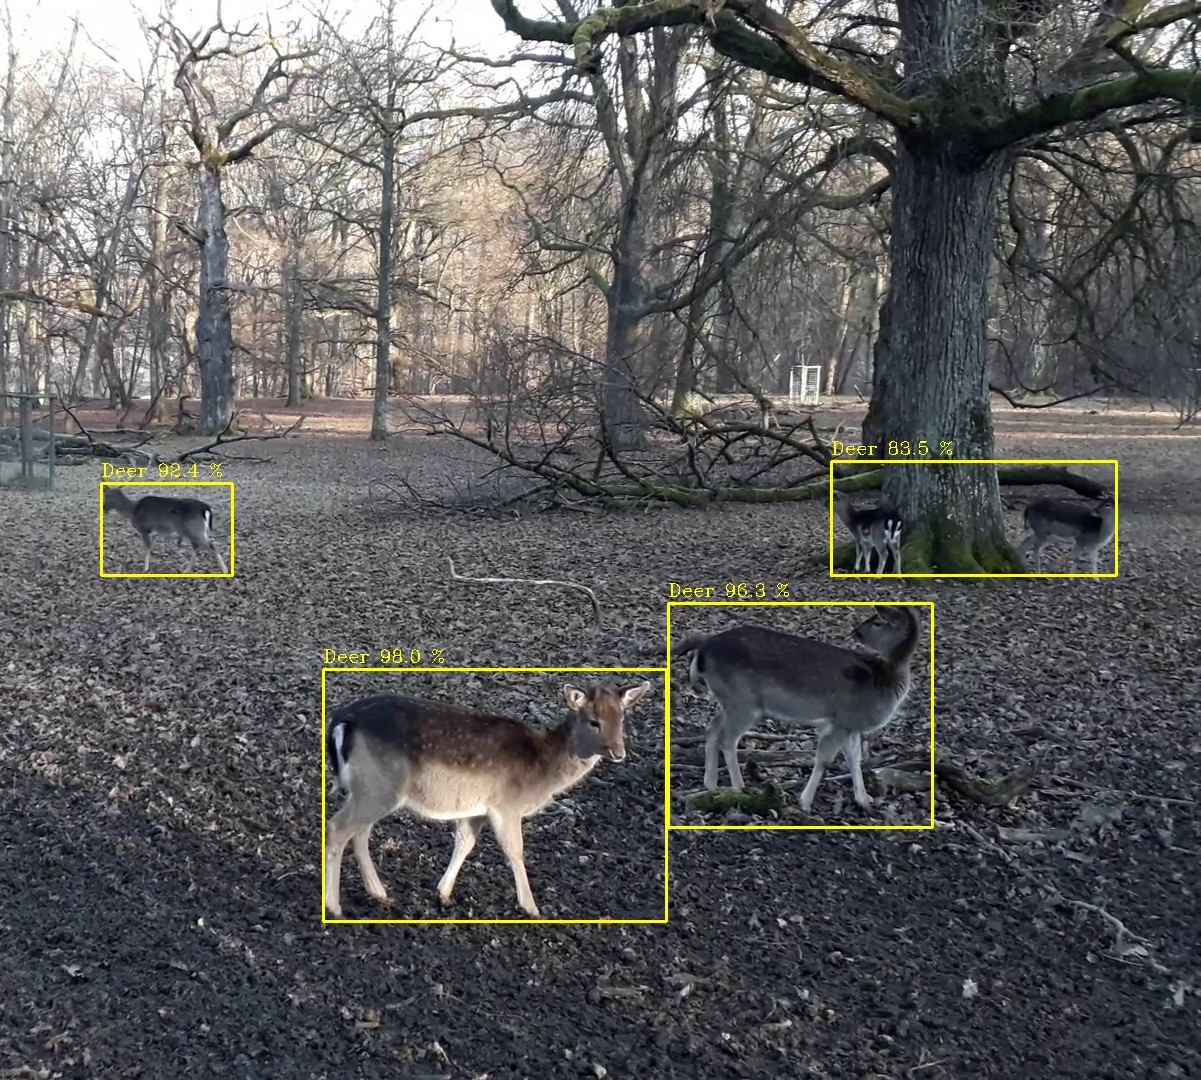
\includegraphics[width=0.9\textwidth]{model_compare_handy_faster_rcnn_inception_v2_early_stopping.jpg}
  \captionof{figure}{Faster R-CNN + Aug}
  \label{}
\end{minipage}


\subsubsection{iWildCam}

Aufnahmen von ... enthällt viele schlecht beleuchtete nacht Aufnahmen 
mit Infrarot Kamera, also ähnlich dem gewünschten Anwendungsfall.
Auch hier erkennt das Faster R-CNN am beste, jedoch 
schneiden hier alle schlecht ab.

Daher wurde, wie im nächsten Abschnitt beschrieben, versuch
das Faster R-CNN noch weiter zu optimieren.


%----------------- SECTION: optimierung ---------------------
\section{Optimierungen: Faster r-CNN}\label{sec:optimierung_faster_rcnn}

Um bessere Ergebnisse für das Faster R-CNN zu erzielen wurde dieses 
nun für mehr durchläufe trainiert. (500k statt 200k)

\subsection{Verschiedene Augmentierungen}

Folgende Plots zeigen Faster R-CNN mit einer Augment pro 
Bildv, zwei Augment pro Bild (3000Samples) und 
zwei Augment pro Bild (4000Samples)
\\[1cm]
\begin{minipage}{0.5\textwidth}
  \centering
  \label{plot:map_diff_aug}
  \def\svgwidth{0.9\textwidth}
  \input{Bilder/plots/diff_aug_map.pdf_tex}
  \captionof{figure}{mAP}
\end{minipage}
\begin{minipage}{0.5\textwidth}
  \centering
  \label{plot:loss_diff_aug}
  \def\svgwidth{0.9\textwidth}
  \input{Bilder/plots/diff_aug_loss.pdf_tex}
  \captionof{figure}{Loss}
\end{minipage}

% Legende
\begin{table}[htb]
  \centering
  \begin{tabular}{m{0.1\textwidth}<{\centering}m{0.2\textwidth}<{\centering}m{0.2\textwidth}<{\centering}}
    $\color[HTML]{CC3311}\medbullet$  Ohne & $\color[HTML]{FF7043}\medbullet$  Early Stopping & $\color[HTML]{0077BB}\medbullet$  Augmentierung
  \end{tabular}    
\end{table}

Mehr Augmentierung führt zu weniger loss, 
jedoch auch schlechterem mAP.


% colors
% orange: FF7043
% blue  : 0077BB
% red   : CC3311



\subsection{Validierung}

Trotz Augmentierung hat das Modell ab 250k schritten overfittet.
Betrachtet man die einzelnen Loss Kurven, aus denen sich der gesammt 
Loss zusammensezt (insgsammt 4 bei faster R-CNN, 2mal rpn, 2mal fully connected am ende)
stellt man fest, dass nur das Rpn netz sich überanpasst.
\\
Da die L2 Regulierung durch anpassung des Config Files für die 
Einstellungen der Model Parameter, auf die Stufen seperat angewendet werden 
kann, wurde diese auf die erste stufe (RPN) mit einem Faktor von 0,001 
angewendet, wodurch sich das Overfitting verhindern ließ.
\\
Auf der anderen Seite hat sich jedoch eine leichte verschlechterung
des mAP ergeben.
\\[1cm]
\begin{minipage}{0.5\textwidth}
  \centering
  \def\svgwidth{0.9\textwidth}
  \input{Bilder/plots/aug_l2_mAP.pdf_tex}
  \captionof{figure}{mAP}
  \label{}
\end{minipage}
\begin{minipage}{0.5\textwidth}
  \centering
  \def\svgwidth{0.9\textwidth}
  \input{Bilder/plots/aug_l2_total_loss.pdf_tex}
  \captionof{figure}{Total Loss}
  \label{}
\end{minipage}
\\[1cm]
\begin{minipage}{0.5\textwidth}
  \centering
  \def\svgwidth{0.9\textwidth}
  \input{Bilder/plots/aug_l2_classifier_loss.pdf_tex}
  \captionof{figure}{Classifier Loss}
  \label{}
\end{minipage}
\begin{minipage}{0.5\textwidth}
  \centering
  \def\svgwidth{0.9\textwidth}
  \input{Bilder/plots/aug_l2_rpn_loss.pdf_tex}
  \captionof{figure}{RPN Loss}
  \label{}
\end{minipage}
\begin{table}[htb]
  \centering
  \begin{tabular}{m{0.3\textwidth}<{\centering}m{0.4\textwidth}<{\centering}}
    $\color[HTML]{CC3311}\medbullet$  nur Augmentierung & $\color[HTML]{0077BB}\medbullet$  Augmentierung+L2 Regulierung
  \end{tabular}    
\end{table}
\\[1cm]
weitere Trainings Konfigurationen waren
\begin{itemize}
  \item dropout
  \item l2 (rpn loss anschauen)
  \item mehr daten (4000 statt 3000)
\end{itemize}
und sind in tabelle so und so dargestellt.

\begin{table}[htb]
  \centering
  \label{table:reg}
  \begin{tabular}{m{0.2\textwidth}|m{0.2\textwidth}<{\centering}m{0.2\textwidth}<{\centering}m{0.2\textwidth}<{\centering}}
  \hline
  \textgreater 400k & mAP  & Loss (Gesammt) & Loss (RPN) \\ \hline\hline
  Augmentierung     & 0,7  & 0,74           &  0,12          \\
  +Dropout          & 0,7  & 0,73           &            \\
  +L2 Reg (0.01)    & 0,7  & 0,69           &            \\
  +L2 Reg (0.02)    & 0,69 & 0,7            &            \\ \hline
  \end{tabular}
  \caption{Regularisierungen}
\end{table}

\subsection{Test Inferenz}

Auf die drei Datensätze um 


\subsection{Graustufen}
da kamerea graustufen bilder liefert, wurde getestet, ob ein 
training in graustufen bilder zu besseren erg führt, ... nicht so.



% \subsection{weitere tabellen}\label{subsec:regularisierung}

% \begin{table}[htb]
%     \centering
%     \label{tab:regularization}
%     \begin{tabular}{| l || c | c | c | c |} 
%         \hline
%         Regularisierung & $mAP_{orig}$ & $mAP_{handy}$ & $Loss_{orig}$ &  $Loss_{handy}$\\
%         \hline
%         Early Stopping (100k steps) & 0.6715 & 0.4265 & 0.6742 & 0.267\\
%         \hline
%         Augmentierung (200k steps) & 0.6914 & 0.4537 & 0.6738 & 0.2503\\ % hier noch verschiedene kombinationen von augmentierungen
%         \hline
%     \end{tabular}        
%     \caption{Regularization}
% \end{table}




% \subsection{Graustufen/Infrarot Bilder}\label{subsec:eval_gray}


% \begin{table}[htb]
%     \centering
%     \label{tab:eval_gray}
%     \begin{tabular}{| l | l || c | c |} 
%         \hline
%         Modell & Dataset & mAP & Loss\\
%         \hline
%         \multirow{2}{*}{rgb} & original & 0.6556 & 0.1451 \\
%         & handy & 0.4155 & 0.2389 \\
%         \hline
%         \multirow{2}{*}{gray 1 channel} & original & 0.5625 & 0.1716 \\
%         & handy & 0.3226 & 0.2747 \\
%         \hline
%         \multirow{2}{*}{gray 3 channel} & original & 0.664 & 0.1653 \\
%         & handy & 0.438 & 0.2492 \\
%         \hline
%     \end{tabular}        
%     \caption{Grayscale}
% \end{table}





\section{Inferenz zeit}

Verglichen wurde, wie viele Frames die verschieden Modelle jeweils, 
pro Sekunde inferieren können. Dafür wurden jeweils 100 Bilder 
inferiert aund daraus die Fps errechnet. 
Ausgefüher wurde auf dem über den raspberry auf dem ncs2.

Es wurden die Asynchrone Inferenz für 1 bis 4 inferenz Requests gemessen.

\begin{table}[hpb]
  \centering
  \begin{tabular}{m{0.25\textwidth}|m{0.1\textwidth}<{\centering}|m{0.1\textwidth}<{\centering}|m{0.1\textwidth}<{\centering}|m{0.1\textwidth}<{\centering}}
  \hline
  \multirow{2}{*}{Model} & \multicolumn{4}{c}{Asynchronge Inferenz Requests} \\ \cline{2-5} 
                         & 1           & 2          & 3          & 4          \\ \hline\hline
  SSD MobilenetV2        & 19,5           & 35,2          & 40,6          & 40,3          \\
  SSD InceptionV2        & 15,6           & 27,7          & 31,1          & 31,7          \\
  Faster R-CNN Incept.   & 0,63           & 0,67          & 0,75          & 0,74          \\ \hline
  \end{tabular}
\end{table}